\documentclass[10pt, a4paper]{beamer}

\usetheme{Berkeley}
\usecolortheme{sidebartab}
\usepackage{graphicx}
\graphicspath{{images/}}

\begin{document}
	\setbeamertemplate{sidebar left}{}
	\title{Progress Presentation-I}
	\subtitle{e-Yantra Summer Internship 2017 \\ \bfseries Control and Algorithms Development for Quadcopters}
	\author{Heethesh Vhavle\\
	Mentors: Sanam Shakya $|$ Pushkar Raj}
	\institute{IIT Bombay}
	\date{\today}
	%\addtobeamertemplate{sidebar left}{}{\includegraphics[scale = 0.3]{logowithtext.png}}
	\frame{\titlepage}

\setbeamertemplate{sidebar left}[sidebar theme]
\section{Overview of Project}
\begin{frame}{Overview of Project}
\bfseries Control and Algorithms Development for Quadcopters \\
\hfill \break
\mdseries The project deals with the study of control algorithms for quadcopter. The goal is to develop custom firmware for quadcopter (or flight controller) for 32-bit microcontrollers such as the CleanFlight firmware on STM32F1xx (ARM Cortex-M3 core). The flight controller is designed to control parameters such as the throttle, yaw, pitch and roll and to develop algorithms considering various motion and dynamics. The next step is to analyse the control algorithm to identify effects of various parameters and to optimize it for stable motion. The final step is to develop a wireless joystick controller for simple maneuvering of the quadcopter. 	
\end{frame}

\section{Overview of Task}
\begin{frame}{Overview of Task}
\bfseries Task 1\\ \mdseries Study of datasheet and user guide of Pluto Drone.\\ \hfill \break
\bfseries Task 2\\ \mdseries Installation and Setup of IDE and tools.\\ \hfill \break
\bfseries Task 3\\ \mdseries Libraries development for GPIO, Timers, PWM, UART, I2C interface.\\
Interfacing IMU to obtain filtered pitch, roll and yaw angles.\\ \hfill \break
\bfseries Task 4\\ \mdseries Code development for control of quadcopter for stable flight.\\ \hfill \break
\bfseries Task 5\\ \mdseries Wireless joystick control (using Node MCU).\\ \hfill \break
\bfseries Task 6\\ \mdseries Documentation for testing and debugging the drone.\\ \hfill \break
\end{frame}

\section{Task Accomplished}
\begin{frame}{Task Accomplished}
\bfseries Task 1\\ Study of datasheet and user guide of Pluto Drone\\ \hfill \break
\mdseries A brief study on the ARM Cortex-M3 architecture was done to understand how the various peripherals (such as the timers, GPIO ports, I2C ports) have been interfaced the APB (Advanced Peripheral Bus) of the STM32F10xx. Study of the clock distribution (RCC) and configuration of various clock sources.\hfill \break

Brief study of existing flight controllers such as CleanFlight  and Naze32 for 32-bit micro-controllers.
\end{frame}

\begin{frame}{Task Accomplished}
\bfseries Task 2\\ Installation and Setup of IDE and tools\\ \hfill \break
\mdseries Successfully installed TrueSTUDIO IDE, GNU ARM Tool-chain, Windows Build Tools, OpenOCD, Device Packs and Drivers for STM32F10xx. Hardware debugging was successfully completed.
\end{frame}

\begin{frame}{Task Accomplished}
\bfseries Task 3\\ Libraries development for GPIO, Timers, PWM, UART, I2C interface\\ \hfill \break
\mdseries Developed libraries for GPIO pin control, configured timers for PWM control of motors, serial communication over UART was successfully achieved for various data types, I2C port was configured and setup for sensor interfacing, with the help HAL drivers.\hfill \break

MPU9250 Accelerometer and Gyroscope was interfaced and libraries were developed for the same. AK8963 Magnetometer was also interfaced. Raw data was successfully obtained and a complimentary filter was implemented to find pitch and roll angles. Finding the yaw angle required a more complex algorithm and this was achieved using Madgwick's AHRS filter. However, the angles obtained are not yet accurate due to certain problems with Accelerometer interfacing.
\end{frame}

\begin{frame}{Task Accomplished}
\bfseries Sensor Calibration and Data Visualization\\ \hfill \break
\mdseries The MPU9250 and AK8963 sensors were calibrated for offsets. The calibrated data was visualized using Python. Currently working on real time data visualization using Python. Successfully implemented data frame transmission with checksum. Process of plotting the real time data and development of a GUI is ongoing.
\end{frame}

\begin{frame}{Task Accomplished}
\begin{center}
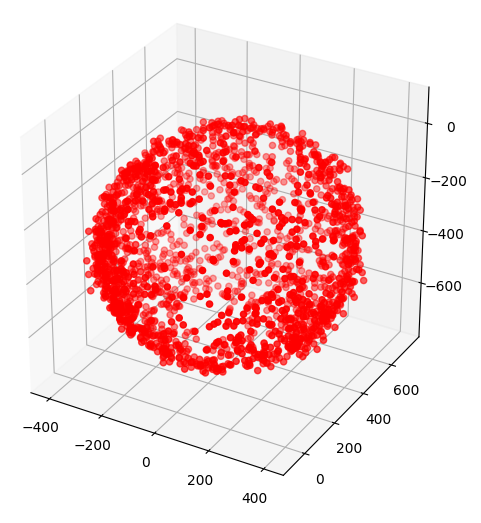
\includegraphics[scale=0.45]{raw}\\
Raw Data from AK8963 Magnetometer
\end{center}
\end{frame}

\begin{frame}{Task Accomplished}
\begin{center}
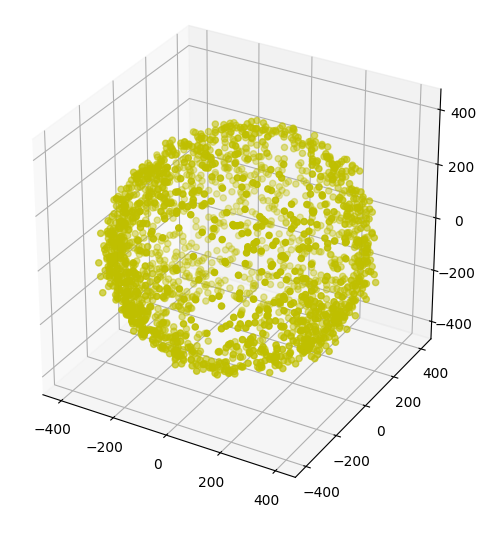
\includegraphics[scale=0.45]{offset}\\
Offset Corrected Data
\end{center}
\end{frame}

\begin{frame}{Task Accomplished}
\begin{center}
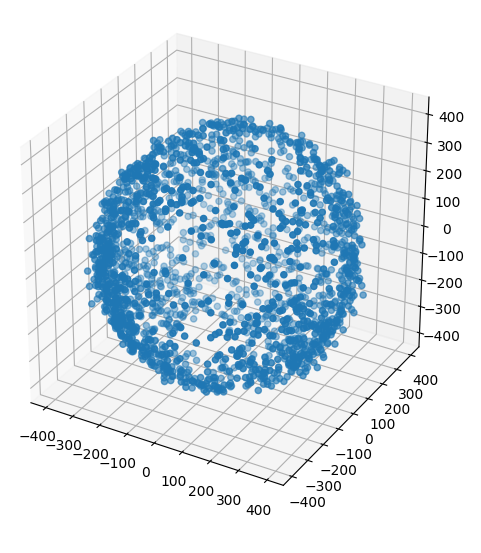
\includegraphics[scale=0.45]{scaled}\\
Scaled and Offset Corrected Data
\end{center}
\end{frame}

\section{Challenges Faced}
\begin{frame}{Challenges Faced}
\begin{itemize}
\item One of the main challenges was developing libraries for peripheral interfaces because of the vast array of documentation and software libraries to wade through [Solved].\\
\item Sensor calibration to obtain accurate data which is required for sensor fusion [Solved].\\
\item Interfacing the AK8963 magnetometer on the same I2C bus as that of the MPU9250 [Solved].\\
\item Abrupt changes in the accelerometer data due to which angles computed are not stable [Debugging].
\end{itemize}
\end{frame}

\section{Future Plans}
\begin{frame}{Future Plans}
\begin{itemize}
\item Perfectly calibrated pitch, roll and yaw with real-time data visualization (with GUI).\\
\item Initial control algorithms for pitch, roll, yaw and throttle control will be developed.\\
\item Barometer and VL53L0X ranging sensor interface for stable altitude control.
\end{itemize}
\end{frame}


\section{Thank You}
\begin{frame}{Thank You}
	\centering THANK YOU !!!
\end{frame}
\end{document}
